\documentclass[]{article}

% Imported Packages
%------------------------------------------------------------------------------
\usepackage{amssymb}
\usepackage{amstext}
\usepackage{amsthm}
\usepackage{amsmath}
\usepackage{enumerate}
\usepackage{fancyhdr}
\usepackage[margin=1in]{geometry}
\usepackage{graphicx}
\usepackage{placeins}
\usepackage{float}
\usepackage{array}
\graphicspath{ {./images/} }
\usepackage{svg}
%\usepackage{extarrows}
%\usepackage{setspace}
%------------------------------------------------------------------------------

% Header and Footer
%------------------------------------------------------------------------------
\pagestyle{plain}  
\renewcommand\headrulewidth{0.4pt}                                      
\renewcommand\footrulewidth{0.4pt}                                    
%------------------------------------------------------------------------------

% Title Details
%------------------------------------------------------------------------------
\title{Deliverable \#2}
\author{SE 3A04: Software Design II -- Large System Design}
\date{}                               
%------------------------------------------------------------------------------

% Document
%------------------------------------------------------------------------------
\begin{document}

\maketitle	
\noindent{\bf Tutorial Number:} T03\\
{\bf Group Number:} G6 \\
{\bf Group Members:} 
\begin{itemize}
	\item Cass Braun
	\item Nehad Shikh Trab
	\item Savvy Liu
	\item Tvesha Shah
	\item Victor Yu
\end{itemize}

\section*{IMPORTANT NOTES}
\begin{itemize}
	%	\item You do \underline{NOT} need to provide a text explanation of each diagram; the diagram should speak for itself
	\item Please document any non-standard notations that you may have used
	\begin{itemize}
		\item \emph{Rule of Thumb}: if you feel there is any doubt surrounding the meaning of your notations, document them
	\end{itemize}
	\item Some diagrams may be difficult to fit into one page
	\begin{itemize}
		\item Ensure that the text is readable when printed, or when viewed at 100\% on a regular laptop-sized screen.
		\item If you need to break a diagram onto multiple pages, please adopt a system of doing so and thoroughly explain how it can be reconnected from one page to the next; if you are unsure about this, please ask about it
	\end{itemize}
	\item Please submit the latest version of Deliverable 1 with Deliverable 2
	\begin{itemize}
		\item Indicate any changes you made.
	\end{itemize}
	\item If you do \underline{NOT} have a Division of Labour sheet, your deliverable will \underline{NOT} be marked
\end{itemize}

\newpage
\section{Introduction}
\label{sec:introduction}
% Begin Section
\subsection{Purpose}
\label{sub:purpose}
% Begin SubSection
This document provides a high-level overview of the Gaim wildlife identification system architecture, including design considerations for the system and its subsystems. The document details architectural choices, subsystem interactions, and class-level responsibilities within the system.\newline

\noindent{The intended audience for this document includes internal stakeholders such as software developers, system architects, project managers, domain experts in wildlife identification, and potential investors interested in the technological aspects of Gaim. It is recommended that Deliverable 1 be reviewed prior to reading this document for a foundational understanding of the system requirements.}
% End SubSection

\subsection{System Description}
\label{sub:system_description}
% Begin SubSection
The system utilizes a Model-View-Controller (MVC) architecture combined with Repository and Blackboard architectural styles to efficiently process data from various knowledge sources and provide accurate species identification.\newline

\noindent{The system is designed to facilitate interactions between different subsystems with some subsystems incorporating blackboard architecture, while other incorporate repository architectural style.}


% End SubSection

\subsection{Overview}
\label{sub:overview}
% Begin SubSection
The remainder of this document is structured as follows:

\begin{itemize}
    \item \textbf{Section 2:} Provides the Analysis Class Diagram for Gaim, illustrating the relationships between key system components.
    \item \textbf{Section 3:} Discusses the overall architectural design of the system, including the rationale behind the chosen architectural styles, the division of the system into subsystems, and their respective functionalities.
    \item \textbf{Section 4:} Presents Class Responsibility Collaboration (CRC) cards, detailing the responsibilities of major classes and their interactions.
\end{itemize}


% End SubSection

% End Section

\section{Analysis Class Diagram}
\label{sec:analysis_class_diagram}
% Begin Section
This section should provide an analysis class diagram for your application.
% End Section


\section{Architectural Design}
\label{sec:architectural_design}
% Begin Section
\subsection{System Architecture}
\label{sub:system_architecture}
% Begin SubSection
The Gaim app utilizes an Interaction-Oriented Software Architecture, specifically Model View Controller, to house all the subsystems. The view represents the interface for user interaction and the controller and model represent the three major subsystems and their respective database. The subsystems follow Data-Centric Architecture styles with classification subsystems using Blackboard. The agents are the independent experts (knowledge sources) with whom the user can interact. Synchronously, the blackboard, the active data store component, will take this information in, dividing the solution space, providing a non-deterministic answer and controlling the logic of the application. \\

\begin{table}[h]
Within our system, the components are defined as the following:  
    \centering
    \renewcommand{\arraystretch}{1.3}
    \begin{tabular}{| m{5cm} | m{6cm} | m{4cm} |}
        \hline
        \textbf{Subsystem} & \textbf{Purpose} & \textbf{Architectural Style} \\
        \hline
        Classification Management & Start a search, submit an image, submit text, fill a survey & Blackboard \\
        \hline
        Generate a Report & View result, generate report, view score, save & Repository \\
        \hline
        Account Management & Create an account and log in to an account & Repository \\
        \hline
    \end{tabular}
    % \caption{Subsystems and Their Architectural Styles}
    % \label{tab:subsystems}
\end{table}

System relationships are defined in section 3.2 of this document. 
\\

Three databases are present on the model level of this architecture. An account database for account details, a classification database with background information regarding species identification (encompassing both description and image sources), and a report generation database to track user-saved searches. 
\\

Our system architecture incorporates the Repository and Blackboard architecture styles. The blackboard style is chosen because it supports multiple independent knowledge sources that can be independently called and allows for a logical data store to present a final output. This is beneficial as our app involves multiple experts/sources of input that the user can utilize, either exclusively or in tandem, to classify a species. Due to this functionality, Blackboard architecture is ideal for classification management as we can narrow down the solution space based on agents and manage them based on the status of the data store. Additionally, in terms of further expansion, it will become very easy to incorporate additional experts/knowledge sources, giving the user more potential use cases for the application.
\\

Another one of the architectures we chose is the Repository Architecture Style as it supports the direct fetching of deterministic outputs from agent requests. This architectural style supports large complex information systems where different components need to access various areas of information. This is the type of access the account management subsystem and report generation system will require, as many users should be able to use the application at the same time and access their specific reports and data. Additionally, this style allows the account management system to easily access stored user information, making it easy for agents to create new accounts and pull credentials for verification. This style also supports data integrity, for backups and restores, which is ideal for account security. Furthermore, for the generated report subsystem, the repository style allows direct access to information from our report generation database and enables the subsystem to display the requested report based on user (agent) input. This architectural style is ideal for expanding new applications, making it easy for us to manage user data, ensure data integrity, and potentially expand the user base.
\\

The overall architecture style chosen for the interaction between these subsystems is the Model View Controller. This architecture style is used because it supports the connection between the user view (presentation) and the data model (backend component) through a controller component that manages input situations and communicates with the appropriate subsystem/database functionality. We can also support frequent data changes, which is essential in the hunting sector which has a changing landscape based on seasonality and new regulations. Further, it is easy to update current functionalities and logic in one component without changing the entire system. This can be beneficial for a newer product because of frequent updates in the user interface or changes to classification logic.  
\\

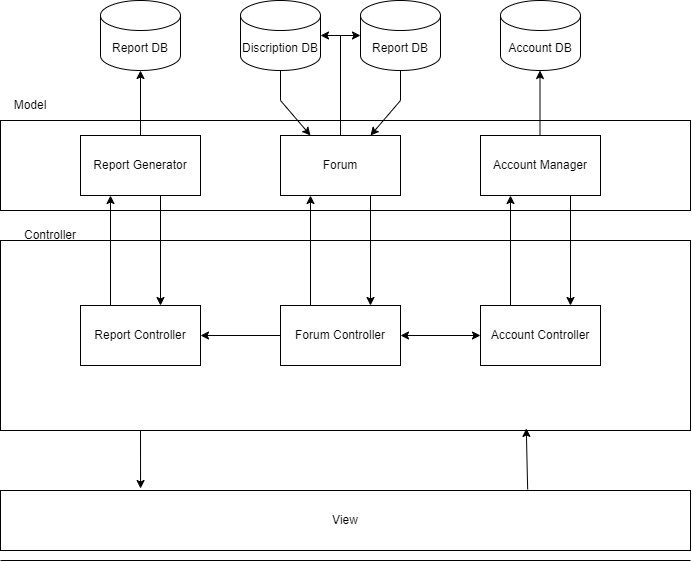
\includegraphics[width=0.6\textwidth]{architecture.png}

% End SubSection
\subsection{Subsystems}
\label{sub:subsystems}
% Begin SubSection
\subsubsection{Classification Management}
The pupose of the Classification Management subsystem is to manage interactions with the user, allowing them to start a search for an animal, and offering various optional input types such as image submission, text submission, and survey submission. It will then interface with both the Report Generation and Account Management submissions to first pass its results and save them to the account history respectively. Overall, it manages the main animal search function of the app, and coordinates these details with the other subsystems.
\subsubsection{Generate Report}
The Generate Report subsystem manages all aspects of the report on the animal guessed. It's primary functions include Allowing the user to view the result of their given input, generating a unique report with details about the result of their search and related information (such as animal age, lifespan, habitat, etc.), viewing the accuracy score of each search, and saving the result which allows the user to store the output of their search.
It interfaces with the Forum subsystem to request search results in order to generate its reports.
\subsubsection{Account Management}
This subsystem manages all aspects of account creation and account interaction including creating an account, logging in to the account, and managing account details such as password resets and interacting with the greater account database. It interfaces with the Classification Management subsystem in order to associate search result details to a specific account as well as allowing access to the Classification Management subsystem itself through logging in.

% End SubSection

% End Section
	
\section{Class Responsibility Collaboration (CRC) Cards}
\label{sec:class_responsibility_collaboration_crc_cards}
% Begin Section

	\begin{table}[H]
	    \centering
	    \begin{tabular}{|p{7cm}|p{7cm}|}
	    \hline 
	     \multicolumn{2}{|l|}{\textbf{Class Name: Success Message (Forum - Boundary)}} \\
	    \hline
	    \textbf{Responsibility:} & \textbf{Collaborators:} \\
	    \hline
	    Knows Forum \newline
	    Displays success message to user upon successful operation \newline
	    Provides feedback on completed processes & 		
	    Forum \\
	    \hline
	    \end{tabular}
	\end{table}
	
	\begin{table}[H]
	    \centering
	    \begin{tabular}{|p{7cm}|p{7cm}|}
	    \hline 
	     \multicolumn{2}{|l|}{\textbf{Class Name: Failure Message (Forum - Boundary)}} \\
	    \hline
	    \textbf{Responsibility:} & \textbf{Collaborators:} \\
	    \hline
	    Knows Forum \newline
	    Displays error message when a process fails \newline
	    Provides guidance on next steps for users & 		
	    Forum \\
	    \hline
	    \end{tabular}
	\end{table}
	
	\begin{table}[H]
	    \centering
	    \begin{tabular}{|p{7cm}|p{7cm}|}
	    \hline 
	     \multicolumn{2}{|l|}{\textbf{Class Name: Login Error (Account - Boundary)}} \\
	    \hline
	    \textbf{Responsibility:} & \textbf{Collaborators:} \\
	    \hline
	    Knows Account Manager \newline
	    Displays login failure message \newline
	    Provides options to reset password or re-enter credentials & 		
	    Account Manager \\
	    \hline
	    \end{tabular}
	\end{table}
	
	\begin{table}[H]
	    \centering
	    \begin{tabular}{|p{7cm}|p{7cm}|}
	    \hline 
	     \multicolumn{2}{|l|}{\textbf{Class Name: Login Success (Account - Boundary)}} \\
	    \hline
	    \textbf{Responsibility:} & \textbf{Collaborators:} \\
	    \hline
	    Knows Account Manager \newline
	    Confirms successful login and redirects user to dashboard \newline
	    Provides session authentication for continued use & 		
	    Account Manager \\
	    \hline
	    \end{tabular}
	\end{table}
	\begin{table}[H]
		\centering
		\begin{tabular}{|p{7cm}|p{7cm}|}
		\hline 
		 \multicolumn{2}{|l|}{\textbf{Class Name: Forum (Controller)}} \\
		\hline
		\textbf{Responsibility:} & \textbf{Collaborators:} \\
		\hline
		Knows Free Form Search \newline
		Knows Survey Search \newline
		Knows Image Search \newline
		Knows Success Message \newline
		Knows Failure Message \newline
		Knows Free Form Agent \newline
		Knows Survey Agent \newline
		Knows Image Agent & 		
		Start Free Form Search \newline
		Start Image Search \newline
		Start Survey Search \newline
		Success Message \newline
		Failure Message \newline
		Free Form Agent \newline
		Survey Agent \newline
		Image Agent \\
		\hline
		\end{tabular}
	\end{table}		
	\begin{table}[H]
		\centering
		\begin{tabular}{|p{7cm}|p{7cm}|}
		\hline 
		 \multicolumn{2}{|l|}{\textbf{Class Name: Start Image Search (Boundary)}} \\
		\hline
		\textbf{Responsibility:} & \textbf{Collaborators:} \\
		\hline
		Knows Forum \newline
		Handles image submission events & Forum \\
		\hline
		\end{tabular}
	\end{table}
	\begin{table}[H]
		\centering
		\begin{tabular}{|p{7cm}|p{7cm}|}
		\hline 
		 \multicolumn{2}{|l|}{\textbf{Class Name: Start Freeform Search (Boundary)}} \\
		\hline
		\textbf{Responsibility:} & \textbf{Collaborators:} \\
		\hline
		Knows Forum \newline
		Handles freeform test submission events & Forum \\
		\hline
		\end{tabular}
	\end{table}
	\begin{table}[H]
		\centering
		\begin{tabular}{|p{7cm}|p{7cm}|}
		\hline 
		 \multicolumn{2}{|l|}{\textbf{Class Name: Start Survey Search (Boundary)}} \\
		\hline
		\textbf{Responsibility:} & \textbf{Collaborators:} \\
		\hline
		Knows Forum \newline
		Handles survey submission events & Forum \\
		\hline
		\end{tabular}
	\end{table}
	\begin{table}[H]
		\centering
		\begin{tabular}{|p{7cm}|p{7cm}|}
		\hline 
		 \multicolumn{2}{|l|}{\textbf{Class Name: Generate Report (Boundary)}} \\
		\hline
		\textbf{Responsibility:} & \textbf{Collaborators:} \\
		\hline
		Knows Report Generator \\
		Knows Report Database & 		
		Forum \\
		Report Generator \\
		Report Database \\
		\hline
		\end{tabular}
	\end{table} 
	
	\begin{table}[H]
		\centering
		\begin{tabular}{|p{7cm}|p{7cm}|}
		\hline 
		 \multicolumn{2}{|l|}{\textbf{Class Name: Report Generator (Controller)}} \\
		\hline
		\textbf{Responsibility:} & \textbf{Collaborators:} \\
		\hline
		Knows Forum \\
		Knows Report Database & 		
		Forum \\
		Report Database \\
		View Reports \\
		\hline
		\end{tabular}
	\end{table} 	
	
	\begin{table}[H]
		\centering
		\begin{tabular}{|p{7cm}|p{7cm}|}
		\hline 
		 \multicolumn{2}{|l|}{\textbf{Class Name: Report Database (Entity)}} \\
		\hline
		\textbf{Responsibility:} & \textbf{Collaborators:} \\
		\hline
		Knows Report Generator \\
		Knows View Reports & 		
		Report Generator \\
		View Reports \\
		\hline
		\end{tabular}
	\end{table}
	
	\begin{table}[H]
		\centering
		\begin{tabular}{|p{7cm}|p{7cm}|}
		\hline 
		 \multicolumn{2}{|l|}{\textbf{Class Name: View Reports (Boundary)}} \\
		\hline
		\textbf{Responsibility:} & \textbf{Collaborators:} \\
		\hline
		Knows Report Database \\
		Knows Report Generator & 		
		Report Database \\
		Report Generator \\
		\hline
		\end{tabular}
	\end{table} 	
	
	\begin{table}[H]
		\centering
		\begin{tabular}{|p{7cm}|p{7cm}|}
		\hline 
		 \multicolumn{2}{|l|}{\textbf{Class Name: Save Report (Boundary)}} \\
		\hline
		\textbf{Responsibility:} & \textbf{Collaborators:} \\
		\hline
		Knows Report Generator & 		
		Report Generator \\
		Report Database \\
		\hline
		\end{tabular}
	\end{table}

	\begin{table}[H]
	    \centering
	    \begin{tabular}{|p{7cm}|p{7cm}|}
	    \hline 
	     \multicolumn{2}{|l|}{\textbf{Class Name: Account Manager (Controller)}} \\
	    \hline
	    \textbf{Responsibility:} & \textbf{Collaborators:} \\
	    \hline
		Knows Login \newline
		Knows Reset Password \newline
		Knows Create Account \newline
		Knows Login Error \newline
		Knows Login Success \newline
		Knows Forum \newline
		Coordinates account interactions from user & 		
	    Login \newline
		Reset Password \newline
		Create Account \newline
		Login Error \newline
		Login Success \newline
		Forum \\
	    \hline
	    \end{tabular}
	\end{table}

	\begin{table}[H]
	    \centering
	    \begin{tabular}{|p{7cm}|p{7cm}|}
	    \hline 
	     \multicolumn{2}{|l|}{\textbf{Class Name: Account Database (Entity)}} \\
	    \hline
	    \textbf{Responsibility:} & \textbf{Collaborators:} \\
	    \hline
	    Knows Account Manager \newline
		Keeps record of all accounts & 		
	    Account Manager \\
	    \hline
	    \end{tabular}
	\end{table}

	\begin{table}[H]
	    \centering
	    \begin{tabular}{|p{7cm}|p{7cm}|}
	    \hline 
	     \multicolumn{2}{|l|}{\textbf{Class Name: Login (Boundary)}} \\
	    \hline
	    \textbf{Responsibility:} & \textbf{Collaborators:} \\
	    \hline
	    Knows Account Manager \newline
		Displays Login Form & 
		Account Manager \\
	    \hline
	    \end{tabular}
	\end{table}

	\begin{table}[H]
	    \centering
	    \begin{tabular}{|p{7cm}|p{7cm}|}
	    \hline 
	     \multicolumn{2}{|l|}{\textbf{Class Name: Reset Password (Boundary)}} \\
	    \hline
	    \textbf{Responsibility:} & \textbf{Collaborators:} \\
	    \hline
	    Knows Account Manager \newline
		Displays reset password form \newline 
		Relays new password information to Account Manager & 		
	    Account Manager \\
	    \hline
	    \end{tabular}
	\end{table}

	\begin{table}[H]
	    \centering
	    \begin{tabular}{|p{7cm}|p{7cm}|}
	    \hline 
	     \multicolumn{2}{|l|}{\textbf{Class Name: Create Account (Boundary)}} \\
	    \hline
	    \textbf{Responsibility:} & \textbf{Collaborators:} \\
	    \hline
		Knows Account Manager \newline
		Displays create account screen \newline
		Runs process to create new account \newline 
		Relays new account information to Account Manager & 		
	    Account Manager \\
	    \hline
	    \end{tabular}
	\end{table}
	
% End Section
\FloatBarrier

\appendix
\section{Division of Labour}
\label{sec:division_of_labour}
% Begin Section
Include a Division of Labour sheet which indicates the contributions of each team member. This sheet must be signed by all team members.
\newline
\newline
\textbf{Cass Braun}
\begin{itemize}
    \setlength\itemindent{2em}
    \item Section 3 - Write description for Generate Report Subsystem
    \item Section 4 - CRC card Account Manager (Controller) 
    \item Section 4 - CRC card Account Database (Entity)
    \item Section 4 - CRC card Login (Boundary)
    \item Section 4 - CRC card Reset Password (Boundary) 
    \item Section 4 - CRC card Create Account (Boundary) \end{itemize} 

\includegraphics[width=0.6\textwidth]{Cass.jpg}

\textbf{Nehad Shikh Trab}
\begin{itemize}
    \setlength\itemindent{2em}
\item Added purpose
\item Added system description
\item Added overview
\item Added Success Message CRC card
\item Added Failure Message CRC card
\item Added Login Error CRC Card
\item Added Login Success CRC Card
\end{itemize}
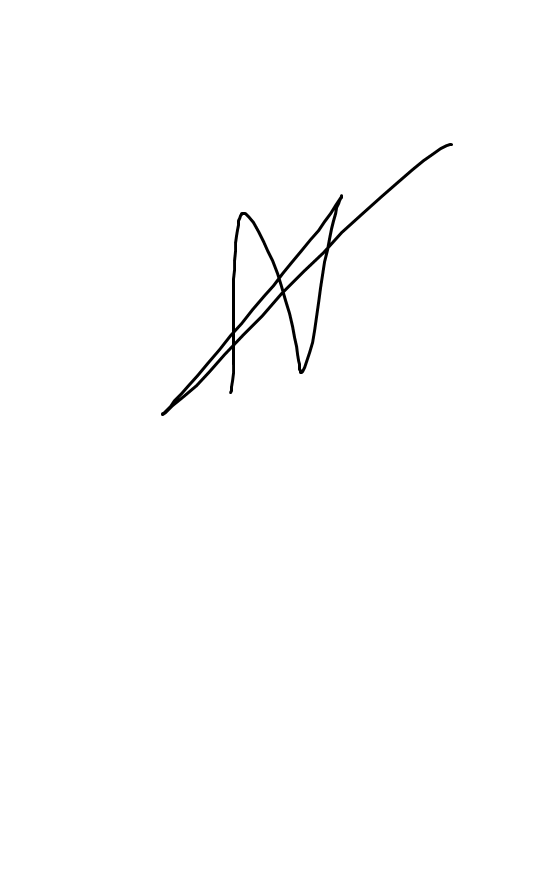
\includegraphics[width=0.6\textwidth]{Nehad.png}

\textbf{Savvy Liu}
\begin{itemize}
\setlength\itemindent{2em}
\item Add contributions 
\end{itemize} 
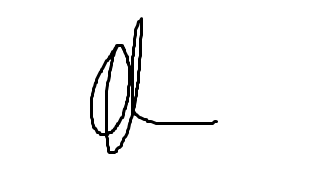
\includegraphics[width=0.6\textwidth]{Savvy.png}

\textbf{Tvesha Shah}
\begin{itemize}
    \setlength\itemindent{2em}
    \item Section 3 -  Identify and explain the overall architecture of your system  
    \item Section 3 - Provide the reasoning and justification of the choice of architecture 
    \item Section 4 - CRC card Forum 
    \item Section 4 - CRC card Start Image Search (Boundary)
    \item Section 4 - CRC card Start Freeform Search (Boundary)
    \item Section 4 - CRC card Start Survey Search (Boundary) 
    \item Managed github set up and assisted with formatting
\end{itemize} 
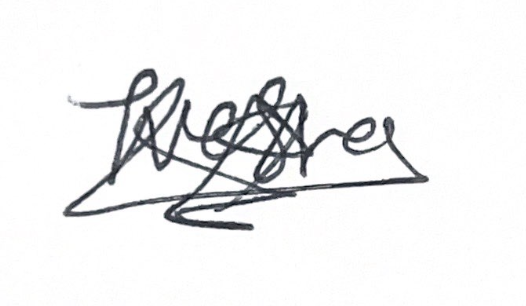
\includegraphics[width=0.6\textwidth]{Tvesha.png}

\textbf{Victor Yu}
\begin{itemize}
    \setlength\itemindent{2em}
\item Add contributions 
\end{itemize}

\includegraphics[width=0.3\textwidth]{Victor.png}
% End Section

\end{document}
%------------------------------------------------------------------------------
